\documentclass{report}
\usepackage[utf8]{inputenc}
\usepackage{graphicx}
\usepackage{verbatim}
\usepackage[siunitx,europeanresistors,americaninductors]{circuitikz}
\usepackage{tikz}
\usepackage{pgfplots}
\usepackage{biblatex}
\usepackage{float}

\title{”Vienkāršu elektrisku shēmu modelēšana”}
\author{Oskars Šēlis}
\date{14.marts 2019}

\begin{document}

\maketitle

\chapter{Teorētiskā daļa}
    Kursa laikā tika apgūtas daudzpusīgas zināšanas elektrisko ķēžu modelēšanā ar dažādām programmām, iemācoties arī iegūt datus no tām, kas attiecīgi tiks apskatīts zemāk. \cite{1}

\begin{circuitikz}[scale=1, every node/.style={transform shape}]
\draw (0,0)
to[V=$U1$, o-o] (0,2)
to[R=$R1$, o-o] (4,2)
to[R=$R2$, *-*] (4,0)
to[short, o-o] (0,0)
;
\end{circuitikz}

\section{Ķēžu aprēķins}
    Zemāk dota tabula ar dotajiem parametriem - rezistoru vērtībām un avotu spriegumu, atrodot simulācijā attiecīgi spriegumu uz rezistoriem R1 un R2.\cite{2}


{\begin{tabular}{ |p{2cm}|p{2cm}| }
\hline
R{1} & 5 \\
\hline
R2 & 7\\
\hline
V1 & 34.6\\
\hline
$U_{R2}$ & 20,18\\
\hline
$U_{R1}$ & 14,42\\
\hline
\end{tabular}



\begin{tikzpicture}[>=latex]
\begin{axis}[
  axis x line=center,
  axis y line=center,
  xtick={-5,0,...,25},
  ytick={-5,0,...,25},
  xlabel={$R$},
  ylabel={$UR$},
  xlabel style={below right},
  ylabel style={above left},
  xmin=0,
  xmax=30,
  ymin=0,
  ymax=30]
\addplot [mark=none,domain=0:25] {sqrt(50*x)};
\end{axis}
\end{tikzpicture}

\chapter{Praktiskā daļa}
Mēs iemācījāmies strādāt ar attiecīgām programmām, lai nosimulētu viemkāršu elektrisku ķēdi

\section{Darbs ar GEDA programmām}
\subsection{Darbs ar gschem}
Šajā programma tika uzmodelēta shēma attiecīgiem aprēķiniem.

\begin{figure}[!h]
\rotatebox{-90}{\includegraphics[width=7cm]{01.ps}}
\caption{1.att.Elektriskā shēma}
\label{fig:01.ps}
Attēls \ref{fig:01.ps} 1.att.gnetlist shēma
\end{figure}

\subsection{Darbs ar gnetlist}
Šī bija otra programma, kurā tika iegūti rezistoru spriegums! Šīs ir programmas izvads, kuri tika ievadīti programmā, modelējot shēmu.
\verbatiminput{01.net}

\subsection{Darbs ar ngspice}
Zemāk redzami grafiki ar izejas spriegumu un spriegumu uz rezistora R2, kas rodas ķēdes iespaidā

\begin{figure}[!H]
\begin{center}
\includegraphics[width=9cm]{011.ps}
\caption{2.att.Grafiks}
\label{fig:01.ps}
\end{center}
\end{figure}
Attēls \ref{fig:011.ps} 2.att.Izejas spriegums

\begin{figure}[!t]
\begin{center}
\includegraphics[width=9cm]{012.ps}
\caption{3.att.Grafiks}
\label{fig:01.ps}
Attēls \ref{fig:012.ps} 3.att.Izejas spriegums
\end{center}
\end{figure}

\section{Darbs ar QUCS programmām}
Trešā programma datu iegūšanai un modelēšanai

\begin{center}
\begin{figure}[!h]
\fbox{\rotatebox{-90}{\includegraphics[width=14cm,trim={0cm 0cm 16cm 24cm}]{print.ps}}}
\caption{4.att.QUCS shēma}
\label{fig:01.ps}
Attēls \ref{fig:print.ps} 4.att.QUCS simulācija
\end{figure}
\end{center}

\begin{figure}[!h]
\begin{center}
\fbox{\rotatebox{-90}{\includegraphics[width=12cm,trim=0cm 0cm 15cm 22cm,clip]{print1.ps}}}
\caption{5.att.QUCS shēma}
\label{fig:01.ps}
Attēls \ref{fig:print1.ps} 5.att.QUCS simulācija
\end{center}
\end{figure}

\begin{figure}[!tb]
\begin{center}
\fbox{\rotatebox{-90}{\includegraphics[width=20cm,trim=1cm 1cm 14cm 24cm,clip]{print_qucs.ps}}}
\caption{6.att.QUCS dati}
\label{fig:01.ps}
Attēls \ref{fig:print_qucs.ps} 6.att.QUCS dati
\end{center}
\end{figure}

\begin{thebibliography}{9}
\bibitem{1}
Rīgas Tehniskās universitātes Elektrotehniskie teorētiskie pamati, Andrejs Strauts, Rīga, 2009.
\bibitem{2}
Rīgas Tehniskās universitātes Elektrotehniskie teor. pamati - lekciju konpekts, Andrejs Strauts, Rīga, 2007
\end{thebibliography}
\end{document}

